%%%%%%%%%%%%%%%%%Epic 12%%%%%%%%%%%%%%%%%%%%%%%%%%%%%%%%%%%%%%%%%%%%%%%%%%%%%%%
\subsection{Ziel erreicht Ausgabe}

Es ist das Ziel, dass der Roboter sicher weiss, dass er sich im Ziel befindet und dies erkenntlich gibt mit einem Buzzer Geräusch.

\subsubsection{Zielknoten erkennen}
\label{detect-target}

Es wurde bereits in \acrshort{pren1} die Methode gewählt, mit welcher die Buchstaben auf den Zielknoten erkannt werden sollen. Dieser Code muss nun lediglich migriert werden, um in die Architektur der Navigation zu passen.

Wie geplant wird der \gls{orb-gloss} Algorithmus verwendet, der in der OpenCV Library vorhanden ist. Es wird die TargetNodeReader Klasse im NodeReader Modul erstellt (siehe Grafik TODO REF WHOLE ARCH). Sobald eine Instanz dieser Klasse erstellt wird, lernt sie die Konturen von den Buchstaben A, B und C und speichert diese in Attributen.
Dies lernt sie von Beispielbildern von den schwarzen Buchstaben auf weissem Hintergrund.
Jedes Mal, wenn der Roboter einen Knoten fotografiert, wird dieses Bild verzerrt, um den Knoten in Vogelperspektive anzuzeigen (siehe Kapitel \ref{outgoing-lines}) und dann wird detektiert, ob sich darauf der Buchstabe des Zielknotens befindet.

Auf folgender Grafik ist die Klasse in Verhältnis zu dem Navigator dargestellt.

\begin{figure}[H]
\centering
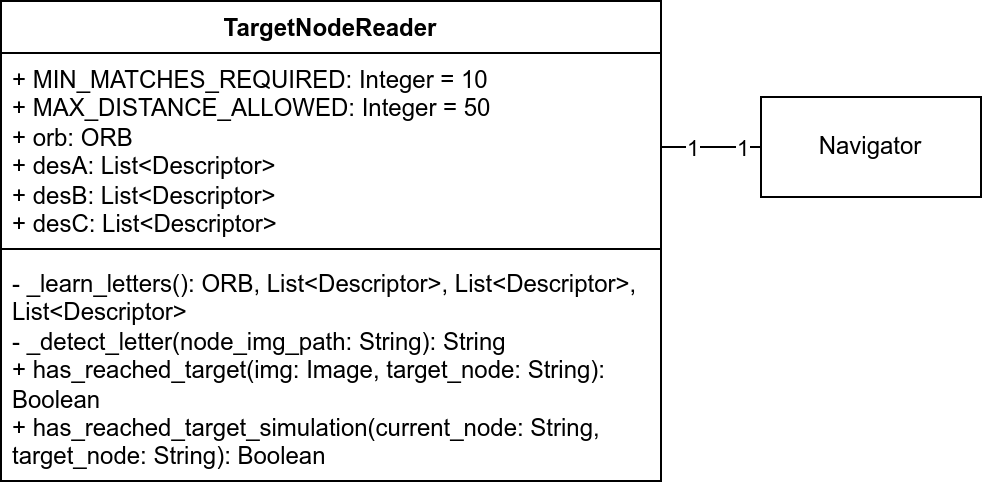
\includegraphics[width=\textwidth]{assets/IT/robot-sw-architecture-target-node-detector.png}
\caption{TargetNodeDetector Klassendiagramm}
\label{fig:target-node-nav}
\end{figure}

\acrshort{orb} gibt jeweils zurück, wie nahe die Anhaltspunkte des richtigen Objektes den Beispielbildern, die er gelernt hat, ist. Damit die Navigation in der Lage ist sowohl den richtigen Buchstaben zu erkennen, als auch jegliche Absenz eines Buchstabens, muss definiert werden, wie sicher der Algorithmus sich sein muss, dass es sich um einen Buchstaben handelt, damit es akzeptiert wird. Dafür wurden die folgenden zwei Parameter definiert:

TODO adjust if tuning
\begin{verbatim}
# Anzahl Anhaltspunkte die gefunden werden müssen
MIN_MATCHES_REQUIRED = 10
# Wie unterschiedlich die Anhaltspunkte sein dürfen,
# um immer noch als Match zu zählen
MAX_DISTANCE_ALLOWED = 50
\end{verbatim}

Diese Funktionalität wurde erneut mit Unittests getestet.
Dabei wird die Klasse, die die Konturen der Buchstaben lernt instanziert und dann werden realistische Bilder an die Methode übergeben, die die Knoten liest. Alle Buchstaben inklusive einem leeren Knoten werden richtig erkannt.

TODO BILDER WENN GEAMACHT

TODO neues RIsiko mitigiert: gibt fälschlich an sei im Ziel obwohl nicht ist -> getestet mit X bildern und immer erkannt

Damit die Navigation nach wie vor auf allen Umgebungen laufen kann, werden hier zwei Methoden erstellt, eine Dummy Methode, die aus dem Simulator übernommen wurde und die richtige Methode, die Buchstaben von Bildern detektiert. so kann einfach hin und her gewechselt werden je nach Umgebung.

\subsubsection{Peripherie - Buzzer}

TODO LUKAS... BUZZER



\newpage
%%%%%%%%%%%%%%%%%Epic 13%%%%%%%%%%%%%%%%%%%%%%%%%%%%%%%%%%%%%%%%%%%%%%%%%%%%%%%
\subsection{Funktion-Stop}

...... POSSIBLY Bild von Schalter

Der Hauptschalter ist benutzerfreundlich ausgeführt und trennt alle für den Fahrbetrieb relevanten Funktionen zuverlässig vom Stromkreis. Befindet sich der Schalter in der unteren Stellung, ist das Fahrzeug vollständig deaktiviert.

Eine Ausnahme bildet der \textit{Raspberry Pi}, der auch bei deaktiviertem Hauptschalter weiterhin mit Strom versorgt wird. Dies ist bewusst so vorgesehen, um Datenverlust oder Dateisystemfehler durch unerwartetes Abschalten zu vermeiden.

...... POSSIBLY Bild von Verkablung
...... POSSIBLY Bild von Verkablungsschema

\subsubsection{Schaltergehäuse}

Am Schaltergehäuse werden Hauptschalter und die zwei Knöpfe TODO IVAN TODO ELIAS (weiss ned wer), WELCHE KNOEPFE montiert. Diese werden zuvorderst auf der Grundplatte angebracht, wo sie einfach zu erreichen sind. Aus dem Gehäuse führen die benötigten Kabel zu den jeweiligen Komponenten.



*CAD-Bild einfügen*

